\section{Introduction}\label{sec:Intro}
In MR imaging, some tissues have poor \emph{contrast}, which means that the boundaries between tissue types cannot be determined.
 To overcome this, particulate solutions of a contrast agent are used to illuminate regions of interest~\cite{na2009inorganic}. 
 Drawbacks include that the contrast agent diffuses quickly and must be injected repeatedly during long scans. 
 Additionally, many contrast agents such as Gadolinium chelates are toxic, and prolonged exposure causes medical complications \cite{caravan1999gadolinium}. 
This paper explores using steerable magnetic microparticles to map a region. 
These particles can be steered by the global magnetic gradient of an MRI and visualised by the MRI \cite{Vartholomeos2012}, even when the tissues they move through  have poor contrast.
As a current example for micro- and nano-particles that can be manufactured in large numbers, see~\cite{Chowdhury2015,martel2014computer,kim2015imparting,Donald2013,Ghosh2009,Ou2013,qiu2015magnetic}.

\begin{figure}
\begin{center}
	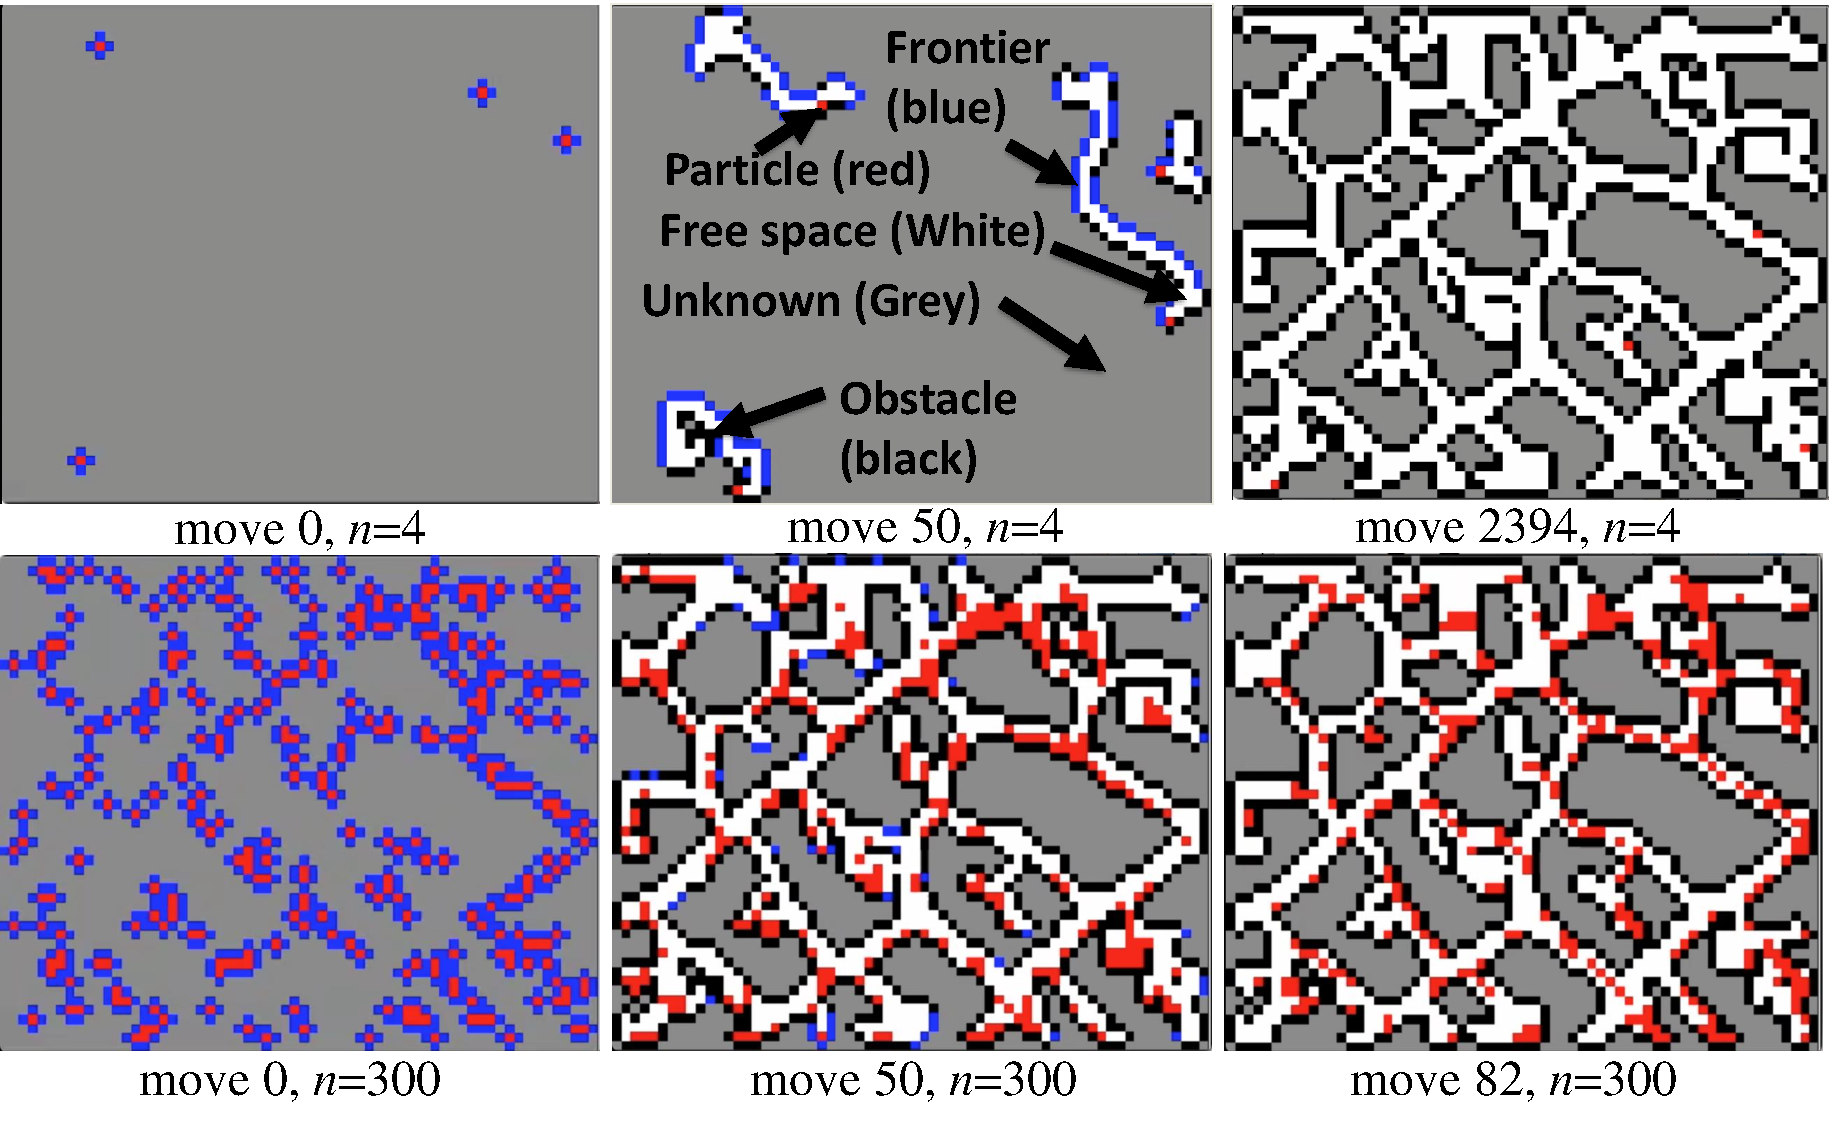
\includegraphics[width=1.0\columnwidth]{Coverage2DwithUnformControl}
\end{center}
\caption{\label{fig:Coverage2DwithUnformControl}
Mapping a 2D environment with 500 blank spaces using $n=4$ (top) and $n=300$ particles, all controlled by an external global force.  After 82 moves, the 300 particles have mapped the entire space, while the 4 particles require a total of 2394 moves to fully map the area. 
}
\end{figure}

The particles considered in this paper move synchronously under the influence of a global command.
They move by the same vector when the force is activated,
unless they get stopped by an obstacle or another stopped particle.  
Using MRI scans, it is possible to detect the location of particles, but not of the presence of tissue;
the key idea is to deduce the presence of obstructing tissue by differences between the expected motion vectors and 
the measured location of particles.

%All particles move in the same direction when commanded. 
In previous work \cite{mahadev2016collecting} we provided an algorithm that guarantees the collection of particles.
 In this work we explore the field of mapping, coverage, and foraging using globally controlled particles. 
 This paper focuses on discrete 2D workspaces.
Fig. \ref{fig:Coverage2DwithUnformControl} represents the complete mapping of a workspace using a large number of particles.  
At the initial step, all  particles (red circles) are in free cells (white squares) and are surrounded by blue squares that represent the unknown frontier cells.
By commanding the particles to take one step in a particular direction, we can categorize the the frontier cell in this direction as either obstacle or free.
 If the particle was able to move, that frontier cell is labelled as free, and new frontier cells are added to adjacent areas that have not been mapped.
 If the particle was unable to move, that frontier cell is labelled as obstacle.
The goal is to explore all  frontier cells, thereby discovering all connected free cells and the obstacles that surround them. 

The paper is arranged as follows. 
After a review of recent related work in Sec.~\ref{sec:RelatedWork}, we introduce the algorithms to perform mapping, coverage, and foraging and also discuss the complexity in Sec.~\ref{sec:theory}.
 In Sec.~\ref{sec:simulation} we discuss the performance of the algorithms on parameters which determine efficiency based on different environments, particle distribution and completion speed. We conclude this paper by summarizing the results and discussing
% Sec.  \ref{sec:expResults} 
 directions for further research in Sec.  \ref{sec:conclusion}.

